\documentclass[10pt]{article}
\usepackage[a4paper,margin=2cm]{geometry}
\usepackage{booktabs,longtable,amsmath,graphicx,pdfpages,caption,lscape}
\captionsetup{font=small,labelfont=bf}
\title{\bfseries Single-Lagrangian CL inflow fits of the SPARC category-A galaxies:\\ fit quality, parameter determination and robustness}
\author{Automated analysis for E.P.J.\ de Haas}\date{}
\begin{document}\maketitle
\section*{Summary}
Of the 175 SPARC galaxies, 54 fall in category A after the single-Lagrangian (single-L) constant-Lagrangian (CL) inflow fit: their weighted residuals show no significant coherent structure (runs test $p\ge0.05$) and $\chi^2_\nu\le1$. For these galaxies the two-parameter CL curve is a statistically complete description of the SPARC rotation curve. The global $\chi^2$ is 100.7 for 341 degrees of freedom ($\chi^2_\nu=0.295$), the median relative RMS residual in $v^2$ is 0.091, and no residual exceeds $2\sigma$. The asymptotic CL speed $v_L=\sqrt{3/2}\,X$ is determined to a median 5.3\%, while $M$ and $R$ individually reach 23\% and 14\% because they are strongly correlated (median $\rho_{MR}=0.967$). The fitted parameters track independent photometric quantities: $v_L$ versus SPARC $V_\mathrm{flat}$ gives $r=0.994$, $\log M$ versus $\log M_\mathrm{bar}$ gives $r=0.81$, and $R$ versus $R_\mathrm{disk}$ gives Spearman $\rho=0.68$. A three-level grading gives 17 galaxies of grade I (both parameters robustly determined), 28 of grade II (asymptotic speed determined, $M$ and $R$ partly degenerate) and 9 of grade III (under-constrained). The main limitation is not the model but the data: category A is dominated by late-type dwarfs with few points (median $n=8$), and the SPARC velocity errors are conservative relative to the scatter about the CL curve, so a good fit here is partly the absence of evidence against the model.

\section{Sample and selection}
Category A was defined in the pipeline run on all 175 SPARC galaxies (Lelli, McGaugh \& Schombert 2016): after the single-L fit, a galaxy is in A when the one-sided Wald--Wolfowitz runs test on the signs of the weighted residuals gives $p_\mathrm{runs}\ge0.05$ (no excess of long same-sign stretches), and $\chi^2_\nu\le1$. Galaxies with a $+-+$ wave (B), a $-+-$ wave (C), other significant structure (D), or $\chi^2_\nu>1$ without structure (E) are excluded.
The selection has three consequences that must be kept in mind. (i) It favours late types: 41 of 54 are Sdm--BCD (median type Sm). (ii) It favours short rotation curves: median $n=8$, only 13 galaxies have $n\ge10$, and 21 have fewer than two points inside the fitted $R$ (8 have none). (iii) It includes all quality classes (18 Q=1, 29 Q=2, 7 Q=3). The runs test has low power for small $n$, so category A membership means \emph{no detectable} structure, not proof that none exists.

\section{Model and methods}
\paragraph{Model.} The single-L CL inflow curve (de Haas, SPARC $H_z$ paper, Eqs.~17--18), with $X=\sqrt{2GM/R}-H_zR$:
\begin{equation*}
v^2(r)=\tfrac12X^2\,r^2/R^2\quad(r\le R),\qquad v^2(r)=\tfrac32X^2-\bigl(\sqrt{2GM/r}-H_zr\bigr)^2\quad(r>R),
\end{equation*}
with $H_z=2.2\times10^{-18}\,\mathrm{s^{-1}}$ fixed, and asymptotic speed $v_L=\sqrt{3/2}\,X$. The fit is to $v^2$ with $\sigma_{v^2}=2V_\mathrm{obs}\,\delta V_\mathrm{obs}$, by bounded least squares from 14 starting radii.
\paragraph{Uncertainties.} Statistical: $1\sigma$ from the local covariance $(J^\mathsf{T}J)^{-1}$; $\sigma_{v_L}$ by linear propagation including the $M$--$R$ covariance. Jackknife: leave-one-out refits, giving a jackknife error and the largest parameter shift in units of $\sigma$. Systematic: the data are refitted with the distance increased by $\delta D$ (radii scale with $D$) and with the inclination increased by $\delta i$ (velocities scale with $1/\sin i$, errors likewise); the two shifts are added in quadrature. SPARC velocity errors exclude both effects.
\paragraph{Fit-quality statistics.} $\chi^2$, $\chi^2_\nu$; the lower-tail probability $P(\chi^2\le\chi^2_\mathrm{obs})$ for $n-2$ degrees of freedom (small values signal overestimated errors); $\mathrm{RMS_{rel}}$ of $(v^2_\mathrm{obs}-v^2_\mathrm{mod})/v^2_\mathrm{obs}$; runs test $p_\mathrm{runs}$; Durbin--Watson statistic DW (2 for uncorrelated residuals); Shapiro--Wilk normality $p_\mathrm{SW}$; fraction of points within $1\sigma$; and $\Delta\mathrm{BIC}_\mathrm{off}$, the BIC change on adding a constant offset $V_0^2$ (2018 RMWRSS variant).
\paragraph{Robustness checks.} The fit is repeated with $H_z=0$ (the 2018 RMWRSS model) to measure the sensitivity to the cosmological term.
\paragraph{Grading.} \textbf{I}: $n\ge8$, at least 2 points inside and 3 outside $R$, $\sigma_M/M\le0.3$, $\sigma_R/R\le0.3$, and no jackknife shift above $2\sigma$. \textbf{II}: not I, but $\sigma_{v_L}/v_L\le0.10$. \textbf{III}: the rest. Galaxies with $P(\chi^2\le\chi^2_\mathrm{obs})<0.01$ are flagged as having conservative errors.

\section{Global fit quality}
\begin{table}[h]\centering\small\caption{Category-A fit-quality statistics (54 galaxies).}\begin{tabular}{lrrrr}\toprule Statistic & 16\% & median & 84\% & range\\\midrule
$n$ & 6 & 8 & 11 & 4--25\\
$\chi^2_\nu$ & 0.039 & 0.177 & 0.656 & 0.004--0.930\\
$P(\chi^2\le\chi^2_\mathrm{obs})$ & 0.000 & 0.020 & 0.320 & 0.000--0.555\\
RMS$_\mathrm{rel}$ & 0.041 & 0.091 & 0.194 & 0.013--0.308\\
$p_\mathrm{runs}$ & 0.089 & 0.202 & 0.582 & 0.051--0.960\\
Durbin--Watson & 0.83 & 1.36 & 2.03 & 0.36--2.86\\
$p_\mathrm{SW}$ & 0.183 & 0.517 & 0.785 & 0.002--1.000\\
fraction $|\mathrm{WR}|\le1$ & 0.88 & 1.00 & 1.00 & 0.67--1.00\\
max $|\mathrm{WR}|$ & 0.31 & 0.68 & 1.23 & 0.08--1.66\\
$\rho_{MR}$ & 0.956 & 0.967 & 0.982 & 0.926--1.000\\
$\sigma_M/M$ & 0.112 & 0.233 & 0.506 & 0.064--1.304\\
$\sigma_R/R$ & 0.074 & 0.139 & 0.317 & 0.043--1.265\\
$\sigma_{v_L}/v_L$ & 0.021 & 0.053 & 0.102 & 0.011--0.383\\
$\Delta$BIC$_\mathrm{off}$ & 0.33 & 1.60 & 2.06 & -3.14--2.91\\
\bottomrule\end{tabular}\end{table}
\paragraph{Residual distribution.} The 449 pooled weighted residuals (Fig.~1) are centred on zero and close to Gaussian in shape, but their dispersion is only 0.47, against 1 expected for correctly scaled errors. After rescaling each galaxy by $\sqrt{\chi^2_\nu}$ the Q--Q plot is linear over $\pm2.5\sigma$. Shapiro--Wilk rejects normality ($p<0.05$) in only 3 galaxies (CamB, F571-V1, UGC 11557), about the 2.7 expected by chance. No residual exceeds $2\sigma$, and only one galaxy has fewer than 68\% of its points within $1\sigma$.

\paragraph{Error calibration.} The lower-tail probability $P(\chi^2\le\chi^2_\mathrm{obs})$ is far from uniform (Fig.~1, right): 32 galaxies lie below 0.05 and 21 below 0.01. With only two free parameters this cannot be overfitting; it means that SPARC's $\delta V_\mathrm{obs}$, which by construction include kinematic asymmetries and non-circular motions, are on average about 1.8 times larger than the scatter of the data about the CL curve. Two consequences follow: $\chi^2_\nu<1$ cannot be used to rank galaxies within category A, and the covariance uncertainties quoted below are conservative.

\paragraph{Residual structure.} By selection $p_\mathrm{runs}\ge0.05$ throughout, but 9 galaxies lie between 0.05 and 0.1 and 18 have DW $<1$. These are the members closest to category B or C and the first candidates for a second Lagrangian if more data become available.

\paragraph{Offset and $H_z$.} No galaxy requires the constant offset: the largest improvement is $\Delta\mathrm{BIC_{off}}=-3.1$ (UGC 6917), and the median is $+1.6$, so the extra parameter is penalised. Setting $H_z=0$ changes $M$ by at most 1.8\% and $R$ by at most 1.3\%. At galactic scales the Hubble term is therefore negligible for the fit, and the 2018 RMWRSS ($H_z=0$) and present fits are equivalent for category A.

\begin{figure}[h]\centering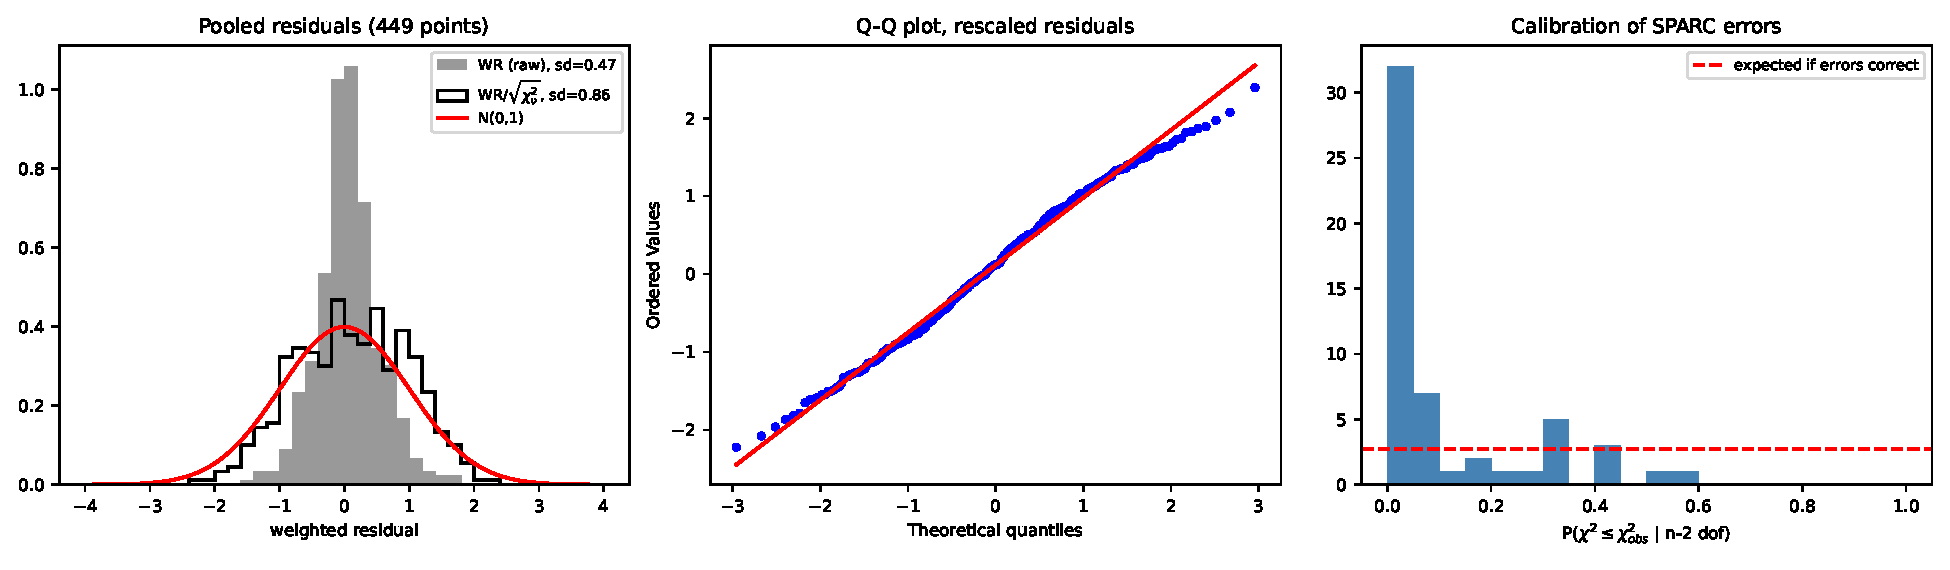
\includegraphics[width=\textwidth]{catA_fig_residuals.pdf}\caption{Left: pooled weighted residuals, raw (grey) and rescaled by $\sqrt{\chi^2_\nu}$ per galaxy (black), against N(0,1). Middle: Q--Q plot of the rescaled residuals. Right: distribution of $P(\chi^2\le\chi^2_\mathrm{obs})$; a uniform distribution (dashed) is expected if the SPARC errors were correctly scaled.}\end{figure}
\section{Parameter determination}
The $M$--$R$ covariance dominates the parameter errors. The correlation coefficient ranges over 0.926--1.000. The data constrain the combination $GM/R$, which sets the plateau $v_L^2\simeq3GM/R$, much better than $M$ and $R$ separately, so solutions slide along lines of constant $v_L$ (Fig.~2, left). Accordingly $v_L$ is the best-determined quantity (median 5.3\%), followed by $R$ (14\%) and $M$ (23\%). $R$ is fixed mainly by where the inner parabola turns over into the outer branch. In the 8 galaxies with no point inside $R$, it is constrained only by the curvature of the outer branch $-2GM/r$, which works but is less precise.

The jackknife errors are smaller than the covariance errors (median ratio 0.61 for $M$), consistent with the conservative SPARC errors. The largest single-point influence exceeds $2\sigma$ in 4 galaxies. The systematic uncertainty from distance and inclination is comparable to the statistical one (median ratio 0.97 for $M$ and 1.14 for $R$), so it should always be quoted alongside it. It matters most for low-inclination galaxies, through the $1/\sin^2 i$ scaling of $v^2$, and for Hubble-flow distances.
\begin{figure}[h]\centering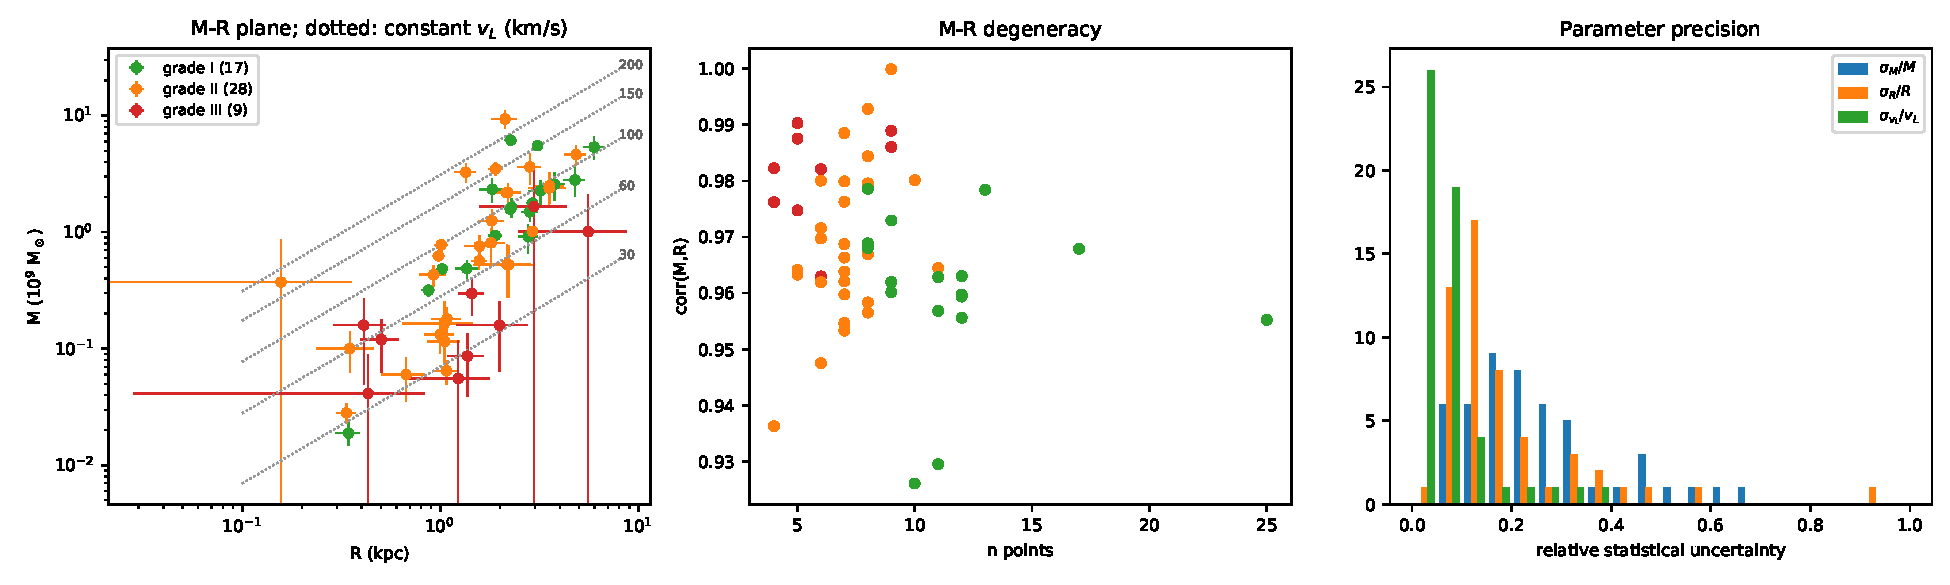
\includegraphics[width=\textwidth]{catA_fig_params.pdf}\caption{Left: fitted $(R,M)$ with $1\sigma$ errors, coloured by grade; dotted lines are curves of constant $v_L$, along which the $M$--$R$ degeneracy runs. Middle: $M$--$R$ correlation versus number of points. Right: relative statistical uncertainties of $M$, $R$ and $v_L$.}\end{figure}
\section{Physical consistency}
For the 28 galaxies with a SPARC $V_\mathrm{flat}$, the CL asymptotic speed tracks it closely ($r=0.994$), with $v_L/V_\mathrm{flat}$ = 1.095 (median). The roughly 10\% excess is expected rather than a bias: at the last measured radius the CL curve has reached only 0.92 of $v_L$ (median), whereas $V_\mathrm{flat}$ is measured from the outermost points. The CL curve therefore predicts a continued slow rise of a few per cent beyond the data, which is a testable prediction for deeper H\,\textsc{i} observations. The fitted mass correlates with the SPARC baryonic mass ($M_\mathrm{bar}=0.5L_\mathrm{disk}+0.7L_\mathrm{bulge}+1.33M_\mathrm{HI}$; $r=0.81$ in log), with median $M/M_\mathrm{bar}=0.41$ (16--84\%: 0.15--0.99). This is much tighter than the $r\approx0.28$ found for the full 175-galaxy sample, and consistent with reading $M$ as the inner (bulge-like) mass rather than the total baryonic mass. $R$ is of the order of the disk scale length (median $R/R_\mathrm{disk}=1.11$, Spearman $\rho=0.68$).
\begin{figure}[h]\centering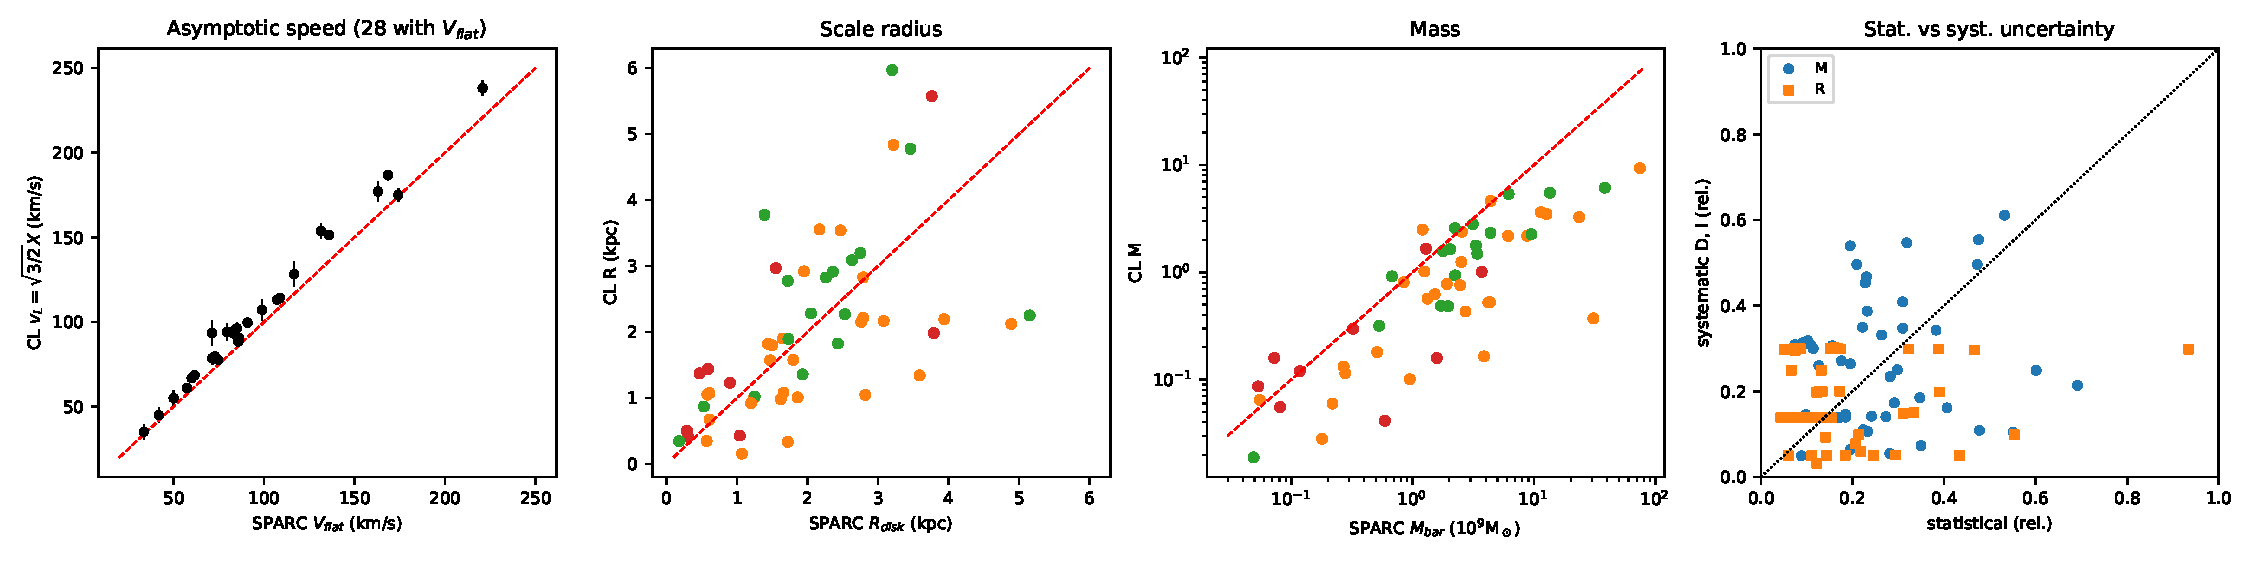
\includegraphics[width=\textwidth]{catA_fig_physics.pdf}\caption{Left to right: CL $v_L$ versus SPARC $V_\mathrm{flat}$; $R$ versus $R_\mathrm{disk}$; $M$ versus $M_\mathrm{bar}$ (dashed: one-to-one); systematic (distance, inclination) versus statistical relative uncertainty of $M$ and $R$.}\end{figure}
\section{Grades and assessment}
\begin{table}[h]\centering\small\caption{Grades (medians per grade).}\begin{tabular}{lrrrrrrr}\toprule Grade & $N$ & $n$ & $\chi^2_\nu$ & RMS$_\mathrm{rel}$ & $\sigma_M/M$ & $\sigma_R/R$ & $\sigma_{v_L}/v_L$\\\midrule
I & 17 & 11 & 0.220 & 0.126 & 0.175 & 0.111 & 0.038\\
II & 28 & 7 & 0.156 & 0.068 & 0.237 & 0.153 & 0.045\\
III & 9 & 5 & 0.082 & 0.143 & 0.692 & 0.390 & 0.174\\
\bottomrule\end{tabular}\end{table}
\textbf{Grade I} (17 galaxies, of which 11 are Q=1) is the core result. The rotation curve samples both the inner parabola and the outer branch, both parameters are determined to better than 30\%, and no single point drives the fit. These are clean, quantitative confirmations that a single constant Lagrangian describes the full rotation curve.
\textbf{Grade II} (28) fits as well statistically, but the data constrain mainly $v_L$. $M$ and $R$ are partly degenerate, usually because of few inner points. These galaxies support the model's plateau and shape but give weaker individual scale parameters.
\textbf{Grade III} (9) are consistent with the model but not informative: with $n\le$ 9 points and parameter errors up to 122\%, almost any smooth rising curve would fit.

\paragraph{Overall assessment.} Within category A the single-L CL model is statistically sufficient. It has no significant residual structure, Gaussian-shaped residuals, no outliers, no need for an offset, and parameters that agree with independent photometric and kinematic scales. Two limitations are intrinsic to the data rather than to the model. First, the SPARC errors are conservative, so goodness of fit cannot discriminate among the A galaxies or between the CL model and other two-parameter models on $\chi^2$ alone. Second, short curves and the $M$--$R$ degeneracy mean that only about a third of the sample (grade I) determines both CL parameters robustly. For comparisons with MOND or dark-matter halos, the grade-I subset with total (statistical plus systematic) uncertainties is the appropriate sample.

\clearpage\begin{landscape}{\scriptsize\setlength{\tabcolsep}{3.5pt}
\begin{longtable}{llrrrrlllllrc}
\caption{Category-A parameters. $R$ in kpc, $M$ in $10^9M_\odot$, $v_L$ in km\,s$^{-1}$. Uncertainties: statistical (covariance) $\pm$ systematic (distance and inclination); jk = jackknife error. $n_\mathrm{in}/n_\mathrm{out}$ = points inside/outside $R$.}\\\toprule
Galaxy & Type & Q & $i$ & $n$ & $n_\mathrm{in}/n_\mathrm{out}$ & $R\pm$stat$\pm$sys & $M\pm$stat$\pm$sys & jk($R$, $M$) & $v_L$ & $\rho_{MR}$ & $V_\mathrm{flat}$ & Grade\\\midrule\endfirsthead
\toprule Galaxy & Type & Q & $i$ & $n$ & $n_\mathrm{in}/n_\mathrm{out}$ & $R\pm$stat$\pm$sys & $M\pm$stat$\pm$sys & jk($R$, $M$) & $v_L$ & $\rho_{MR}$ & $V_\mathrm{flat}$ & Grade\\\midrule\endhead\bottomrule\endfoot
F563--V2 & Im & 1 & 29 & 10 & 3/7 & $1.825\pm0.244\pm0.363$ & $2.33\pm0.53\pm1.1$ & 0.052, 0.17 & $128.2\pm7.4$ & 0.926 & 116.6 & I\\
F583--1 & Sm & 1 & 63 & 25 & 10/15 & $2.915\pm0.192\pm0.725$ & $1.78\pm0.22\pm0.46$ & 0.14, 0.16 & $88.4\pm2.9$ & 0.955 & 85.8 & I\\
F583--4 & Sc & 1 & 55 & 12 & 3/9 & $1.360\pm0.175\pm0.272$ & $0.487\pm0.085\pm0.13$ & 0.32, 0.15 & $67.9\pm2.1$ & 0.960 & -- & I\\
NGC3877 & Sc & 2 & 76 & 13 & 2/11 & $2.268\pm0.166\pm0.314$ & $6.15\pm0.61\pm0.85$ & 0.054, 0.21 & $186.8\pm3.0$ & 0.978 & 168.4 & I\\
NGC3917 & Scd & 1 & 79 & 17 & 3/14 & $3.088\pm0.134\pm0.427$ & $5.51\pm0.35\pm0.76$ & 0.092, 0.22 & $151.5\pm1.9$ & 0.968 & 135.9 & I\\
UGC04483 & Im & 2 & 58 & 8 & 2/6 & $0.344\pm0.049\pm0.032$ & $0.0189\pm0.0042\pm0.0021$ & 0.0096, 0.0011 & $26.6\pm1.2$ & 0.968 & -- & I\\
UGC04499 & Sdm & 1 & 50 & 9 & 2/7 & $1.893\pm0.137\pm0.565$ & $0.935\pm0.1\pm0.29$ & 0.14, 0.098 & $79.7\pm1.7$ & 0.962 & 72.8 & I\\
UGC05005 & Im & 1 & 41 & 11 & 4/7 & $5.968\pm0.723\pm1.178$ & $5.36\pm1.2\pm1.9$ & 0.51, 0.67 & $107.2\pm6.3$ & 0.930 & 98.9 & I\\
UGC05750 & Sdm & 1 & 64 & 11 & 5/6 & $4.775\pm0.582\pm0.945$ & $2.8\pm0.79\pm0.66$ & 0.17, 0.24 & $86.6\pm7.3$ & 0.957 & -- & I\\
UGC06399 & Sm & 1 & 75 & 9 & 2/7 & $2.280\pm0.265\pm0.316$ & $1.64\pm0.3\pm0.23$ & 0.21, 0.22 & $96.2\pm3.7$ & 0.973 & 85.0 & I\\
UGC06667 & Scd & 1 & 89 & 9 & 2/7 & $2.251\pm0.152\pm0.311$ & $1.58\pm0.17\pm0.22$ & 0.3, 0.31 & $94.9\pm2.3$ & 0.960 & 83.8 & I\\
UGC06818 & Sm & 2 & 75 & 8 & 4/4 & $3.774\pm0.451\pm0.522$ & $2.58\pm0.7\pm0.36$ & 0.29, 0.43 & $93.5\pm7.5$ & 0.969 & 71.2 & I\\
UGC07089 & Sdm & 2 & 80 & 12 & 3/9 & $2.826\pm0.272\pm0.391$ & $1.49\pm0.25\pm0.21$ & 0.38, 0.33 & $82.2\pm3.4$ & 0.959 & -- & I\\
UGC07151 & Scd & 1 & 90 & 11 & 2/9 & $1.021\pm0.061\pm0.050$ & $0.483\pm0.043\pm0.024$ & 0.088, 0.055 & $78.0\pm1.3$ & 0.963 & 73.5 & I\\
UGC07603 & Sd & 1 & 78 & 12 & 2/10 & $0.871\pm0.067\pm0.261$ & $0.317\pm0.036\pm0.095$ & 0.083, 0.039 & $68.5\pm1.5$ & 0.963 & 61.6 & I\\
UGC08837 & Im & 2 & 80 & 8 & 5/3 & $2.773\pm0.307\pm0.138$ & $0.915\pm0.26\pm0.05$ & 0.13, 0.13 & $65.0\pm5.7$ & 0.979 & -- & I\\
UGC11557 & Sdm & 2 & 30 & 12 & 5/7 & $3.198\pm0.421\pm0.795$ & $2.26\pm0.52\pm1.1$ & 0.17, 0.21 & $95.3\pm5.3$ & 0.956 & -- & I\\
D512--2 & Im & 2 & 56 & 4 & 1/3 & $0.997\pm0.165\pm0.298$ & $0.132\pm0.041\pm0.046$ & 0.076, 0.015 & $41.3\pm3.4$ & 0.936 & -- & II\\
D564--8 & Im & 2 & 63 & 6 & 2/4 & $1.074\pm0.131\pm0.034$ & $0.0647\pm0.015\pm0.0069$ & 0.065, 0.0066 & $27.8\pm1.7$ & 0.948 & -- & II\\
DDO170 & Im & 2 & 66 & 8 & 1/7 & $2.918\pm0.151\pm0.868$ & $1.02\pm0.075\pm0.31$ & 0.21, 0.098 & $66.8\pm0.9$ & 0.980 & 60.0 & II\\
F561--1 & Sm & 3 & 24 & 6 & 1/5 & $2.217\pm0.741\pm0.331$ & $0.524\pm0.25\pm0.26$ & 0.054, 0.022 & $55.1\pm4.4$ & 0.980 & 50.0 & II\\
F565--V2 & Im & 2 & 60 & 7 & 2/5 & $3.557\pm0.611\pm0.711$ & $2.5\pm0.74\pm0.63$ & 0.12, 0.17 & $94.9\pm6.5$ & 0.969 & -- & II\\
F567--2 & Sm & 3 & 20 & 5 & 1/4 & $2.167\pm0.673\pm0.322$ & $0.527\pm0.25\pm0.29$ & 0.95, 0.27 & $55.8\pm5.4$ & 0.964 & -- & II\\
F571--V1 & Sd & 2 & 30 & 7 & 1/6 & $3.540\pm0.756\pm0.351$ & $2.38\pm0.74\pm0.97$ & 0.15, 0.15 & $92.9\pm5.1$ & 0.976 & 83.6 & II\\
NGC3949 & Sbc & 2 & 55 & 7 & 0/7 & $1.343\pm0.166\pm0.186$ & $3.27\pm0.6\pm0.48$ & 0.072, 0.23 & $177.0\pm6.0$ & 0.980 & 163.0 & II\\
NGC3953 & Sbc & 1 & 62 & 8 & 0/8 & $2.122\pm0.302\pm0.294$ & $9.34\pm1.6\pm1.3$ & 0.34, 1.8 & $238.1\pm4.5$ & 0.993 & 220.8 & II\\
NGC4085 & Sc & 2 & 82 & 7 & 2/5 & $1.901\pm0.154\pm0.264$ & $3.49\pm0.46\pm0.48$ & 0.1, 0.27 & $153.8\pm4.4$ & 0.962 & 131.5 & II\\
NGC4389 & Sbc & 3 & 50 & 6 & 3/3 & $2.828\pm0.387\pm0.392$ & $3.63\pm1.1\pm0.63$ & 0.61, 1.5 & $128.4\pm10.4$ & 0.970 & -- & II\\
UGC02259 & Sdm & 2 & 41 & 8 & 0/8 & $0.980\pm0.073\pm0.289$ & $0.625\pm0.057\pm0.2$ & 0.19, 0.15 & $90.6\pm1.0$ & 0.984 & 86.2 & II\\
UGC04325 & Sm & 1 & 41 & 8 & 1/7 & $1.010\pm0.074\pm0.302$ & $0.778\pm0.08\pm0.25$ & 0.078, 0.077 & $99.6\pm1.8$ & 0.967 & 90.9 & II\\
UGC05414 & Im & 1 & 55 & 6 & 2/4 & $1.570\pm0.135\pm0.469$ & $0.567\pm0.088\pm0.17$ & 0.13, 0.09 & $68.1\pm2.6$ & 0.962 & -- & II\\
UGC05918 & Im & 2 & 46 & 8 & 1/7 & $1.079\pm0.182\pm0.323$ & $0.18\pm0.047\pm0.06$ & 0.073, 0.019 & $46.3\pm2.6$ & 0.957 & -- & II\\
UGC05999 & Im & 2 & 22 & 5 & 1/4 & $4.835\pm0.594\pm0.957$ & $4.62\pm0.9\pm2.5$ & 0.088, 0.14 & $110.6\pm4.6$ & 0.963 & -- & II\\
UGC06628 & Sm & 2 & 20 & 7 & 0/7 & $1.046\pm0.406\pm0.312$ & $0.165\pm0.088\pm0.1$ & 0.17, 0.032 & $45.0\pm4.5$ & 0.954 & 41.8 & II\\
UGC06917 & Sm & 1 & 56 & 11 & 1/10 & $2.152\pm0.142\pm0.298$ & $2.18\pm0.21\pm0.32$ & 0.36, 0.5 & $114.2\pm2.2$ & 0.964 & 108.7 & II\\
UGC06923 & Im & 2 & 65 & 6 & 1/5 & $1.819\pm0.269\pm0.252$ & $1.25\pm0.3\pm0.18$ & 0.58, 0.51 & $94.0\pm4.9$ & 0.972 & 79.6 & II\\
UGC06930 & Sd & 1 & 32 & 10 & 1/9 & $2.194\pm0.337\pm0.303$ & $2.19\pm0.43\pm0.58$ & 0.25, 0.31 & $113.2\pm3.0$ & 0.980 & 107.2 & II\\
UGC06973 & Sab & 3 & 71 & 9 & 0/9 & $0.157\pm0.199\pm0.022$ & $0.373\pm0.49\pm0.053$ & 0.086, 0.21 & $175.0\pm3.7$ & 1.000 & 174.2 & II\\
UGC07261 & Sdm & 2 & 30 & 7 & 0/7 & $0.922\pm0.140\pm0.276$ & $0.431\pm0.09\pm0.21$ & 0.17, 0.1 & $77.6\pm3.1$ & 0.953 & 74.7 & II\\
UGC07559 & Im & 2 & 61 & 7 & 2/5 & $1.051\pm0.193\pm0.053$ & $0.115\pm0.04\pm0.0084$ & 0.097, 0.016 & $37.5\pm3.4$ & 0.960 & -- & II\\
UGC07608 & Im & 1 & 25 & 8 & 3/5 & $1.801\pm0.313\pm0.538$ & $0.809\pm0.26\pm0.44$ & 0.19, 0.16 & $76.0\pm6.1$ & 0.958 & -- & II\\
UGC07690 & Im & 2 & 41 & 7 & 0/7 & $0.349\pm0.113\pm0.104$ & $0.101\pm0.039\pm0.034$ & 0.29, 0.086 & $61.0\pm2.4$ & 0.989 & 57.4 & II\\
UGC07866 & Im & 2 & 44 & 7 & 2/5 & $0.671\pm0.165\pm0.034$ & $0.0598\pm0.024\pm0.0096$ & 0.098, 0.015 & $33.9\pm3.2$ & 0.955 & -- & II\\
UGC10310 & Sm & 1 & 34 & 7 & 1/6 & $1.578\pm0.253\pm0.476$ & $0.758\pm0.18\pm0.29$ & 0.16, 0.098 & $78.6\pm3.4$ & 0.966 & 71.4 & II\\
UGCA281 & BCD & 3 & 67 & 7 & 2/5 & $0.335\pm0.037\pm0.017$ & $0.0281\pm0.0055\pm0.0018$ & 0.037, 0.0047 & $32.9\pm1.5$ & 0.964 & -- & II\\
CamB & Im & 2 & 65 & 9 & 7/2 & $1.373\pm0.283\pm0.106$ & $0.0865\pm0.048\pm0.009$ & 0.2, 0.031 & $28.4\pm4.9$ & 0.989 & -- & III\\
F563--V1 & Im & 3 & 60 & 6 & 1/5 & $1.983\pm0.774\pm0.393$ & $0.159\pm0.096\pm0.04$ & 0.21, 0.035 & $32.0\pm3.9$ & 0.963 & -- & III\\
F574--2 & Sm & 3 & 30 & 5 & 2/3 & $5.572\pm3.082\pm0.550$ & $1.01\pm1.1\pm0.41$ & 0.97, 0.33 & $47.9\pm13.7$ & 0.975 & -- & III\\
NGC4068 & Im & 2 & 44 & 6 & 3/3 & $1.440\pm0.206\pm0.072$ & $0.297\pm0.1\pm0.055$ & 0.14, 0.088 & $51.5\pm5.4$ & 0.982 & -- & III\\
NGC6789 & BCD & 2 & 43 & 4 & 2/2 & $0.410\pm0.121\pm0.021$ & $0.159\pm0.11\pm0.034$ & 0.17, 0.15 & $70.7\pm14.4$ & 0.982 & -- & III\\
UGC02023 & Im & 2 & 19 & 5 & 3/2 & $2.966\pm1.383\pm0.879$ & $1.66\pm2\pm1$ & 0.67, 0.81 & $84.7\pm32.4$ & 0.988 & -- & III\\
UGC07232 & Im & 2 & 59 & 4 & 2/2 & $0.504\pm0.110\pm0.030$ & $0.12\pm0.057\pm0.013$ & 0.14, 0.077 & $55.3\pm7.4$ & 0.976 & -- & III\\
UGC07577 & Im & 2 & 63 & 9 & 6/3 & $1.230\pm0.533\pm0.061$ & $0.0556\pm0.061\pm0.0039$ & 0.24, 0.027 & $24.0\pm8.1$ & 0.986 & -- & III\\
UGC09992 & Im & 2 & 30 & 5 & 0/5 & $0.431\pm0.403\pm0.129$ & $0.0414\pm0.047\pm0.02$ & 0.099, 0.011 & $35.1\pm4.3$ & 0.990 & 33.6 & III\\
\end{longtable}
\begin{longtable}{lrrrrrrrrrrrrc}
\caption{Category-A goodness of fit. $P_<=P(\chi^2\le\chi^2_\mathrm{obs})$; DW = Durbin--Watson; $f_{1\sigma}$ = fraction of points with $|\mathrm{WR}|\le1$; jk$_\mathrm{max}$ = largest leave-one-out shift of $M$ or $R$ in $\sigma$; $\Delta$BIC$_\mathrm{off}$ for an added constant offset; c = conservative-error flag ($P_<<0.01$).}\\\toprule
Galaxy & $n$ & $\chi^2$ & $\chi^2_\nu$ & $P_<$ & AIC & BIC & RMS$_\mathrm{rel}$ & $p_\mathrm{runs}$ & DW & $p_\mathrm{SW}$ & $f_{1\sigma}$ & jk$_\mathrm{max}$ & $\Delta$BIC$_\mathrm{off}$ / flag\\\midrule\endfirsthead
\toprule Galaxy & $n$ & $\chi^2$ & $\chi^2_\nu$ & $P_<$ & AIC & BIC & RMS$_\mathrm{rel}$ & $p_\mathrm{runs}$ & DW & $p_\mathrm{SW}$ & $f_{1\sigma}$ & jk$_\mathrm{max}$ & $\Delta$BIC$_\mathrm{off}$ / flag\\\midrule\endhead\bottomrule\endfoot
F563--V2 & 10 & 0.26 & 0.032 & 0.000 & 4.26 & 4.86 & 0.048 & 0.163 & 1.90 & 0.225 & 1.00 & 0.26 & +2.30 c\\
F583--1 & 25 & 4.90 & 0.213 & 0.000 & 8.90 & 11.33 & 0.250 & 0.059 & 0.82 & 0.605 & 1.00 & 0.40 & +2.91 c\\
F583--4 & 12 & 5.59 & 0.559 & 0.152 & 9.59 & 10.56 & 0.239 & 0.126 & 0.52 & 0.658 & 0.92 & 1.89 & +1.70 \\
NGC3877 & 13 & 1.60 & 0.146 & 0.001 & 5.60 & 6.73 & 0.062 & 0.076 & 0.53 & 0.528 & 1.00 & 0.25 & +2.30 c\\
NGC3917 & 17 & 5.97 & 0.398 & 0.020 & 9.97 & 11.64 & 0.040 & 0.165 & 1.01 & 0.272 & 0.94 & 0.55 & +2.83 \\
UGC04483 & 8 & 1.03 & 0.171 & 0.015 & 5.03 & 5.19 & 0.188 & 0.582 & 1.87 & 0.079 & 1.00 & 0.20 & +1.85 \\
UGC04499 & 9 & 2.44 & 0.348 & 0.068 & 6.44 & 6.83 & 0.100 & 0.051 & 0.76 & 0.506 & 1.00 & 1.06 & +1.16 \\
UGC05005 & 11 & 1.74 & 0.194 & 0.005 & 5.74 & 6.54 & 0.278 & 0.074 & 0.85 & 0.268 & 1.00 & 0.65 & +1.84 c\\
UGC05750 & 11 & 0.33 & 0.036 & 0.000 & 4.33 & 5.12 & 0.065 & 0.225 & 1.60 & 0.734 & 1.00 & 0.17 & +2.40 c\\
UGC06399 & 9 & 1.54 & 0.220 & 0.019 & 5.54 & 5.93 & 0.111 & 0.051 & 1.21 & 0.843 & 1.00 & 0.66 & +1.56 \\
UGC06667 & 9 & 5.01 & 0.716 & 0.342 & 9.01 & 9.41 & 0.145 & 0.110 & 1.35 & 0.410 & 0.67 & 1.84 & -1.08 \\
UGC06818 & 8 & 4.10 & 0.684 & 0.337 & 8.10 & 8.26 & 0.274 & 0.223 & 1.19 & 0.582 & 0.88 & 0.58 & +0.04 \\
UGC07089 & 12 & 7.05 & 0.705 & 0.279 & 11.05 & 12.02 & 0.199 & 0.113 & 0.77 & 0.999 & 0.75 & 1.14 & -1.64 \\
UGC07151 & 11 & 4.01 & 0.445 & 0.089 & 8.01 & 8.80 & 0.070 & 0.225 & 1.59 & 0.338 & 1.00 & 1.41 & +1.37 \\
UGC07603 & 12 & 4.64 & 0.464 & 0.086 & 8.64 & 9.61 & 0.126 & 0.113 & 1.20 & 1.000 & 0.83 & 1.01 & -0.01 \\
UGC08837 & 8 & 0.31 & 0.052 & 0.001 & 4.31 & 4.47 & 0.041 & 0.223 & 1.75 & 0.499 & 1.00 & 0.51 & +2.05 c\\
UGC11557 & 12 & 1.83 & 0.183 & 0.003 & 5.83 & 6.80 & 0.308 & 0.179 & 1.59 & 0.020 & 0.92 & 0.31 & +2.44 c\\
D512--2 & 4 & 0.13 & 0.067 & 0.065 & 4.13 & 2.91 & 0.055 & 0.500 & 2.22 & 0.783 & 1.00 & 0.59 & +1.39 \\
D564--8 & 6 & 0.62 & 0.155 & 0.039 & 4.62 & 4.20 & 0.092 & 0.181 & 1.17 & 0.560 & 1.00 & 0.48 & +1.38 \\
DDO170 & 8 & 2.99 & 0.498 & 0.190 & 6.99 & 7.15 & 0.076 & 0.937 & 2.60 & 0.151 & 1.00 & 1.41 & +1.10 \\
F561--1 & 6 & 0.05 & 0.012 & 0.000 & 4.05 & 3.63 & 0.021 & 0.500 & 2.23 & 0.557 & 1.00 & 0.07 & +1.79 c\\
F565--V2 & 7 & 0.22 & 0.044 & 0.001 & 4.22 & 4.11 & 0.085 & 0.113 & 0.97 & 0.597 & 1.00 & 0.22 & +1.87 c\\
F567--2 & 5 & 0.44 & 0.145 & 0.067 & 4.44 & 3.65 & 0.089 & 0.744 & 2.63 & 0.217 & 1.00 & 1.70 & +1.57 \\
F571--V1 & 7 & 0.20 & 0.039 & 0.001 & 4.20 & 4.09 & 0.060 & 0.358 & 1.66 & 0.046 & 1.00 & 0.14 & +1.87 c\\
NGC3949 & 7 & 0.14 & 0.029 & 0.000 & 4.14 & 4.04 & 0.019 & 0.358 & 2.07 & 0.428 & 1.00 & 0.48 & +1.95 c\\
NGC3953 & 8 & 3.14 & 0.524 & 0.209 & 7.14 & 7.30 & 0.048 & 0.075 & 0.66 & 0.613 & 0.88 & 1.19 & +2.08 \\
NGC4085 & 7 & 0.67 & 0.134 & 0.015 & 4.67 & 4.56 & 0.038 & 0.560 & 1.96 & 0.158 & 1.00 & 0.70 & +1.91 \\
NGC4389 & 6 & 2.98 & 0.745 & 0.439 & 6.98 & 6.56 & 0.176 & 0.181 & 1.17 & 0.241 & 1.00 & 1.09 & +0.55 \\
UGC02259 & 8 & 3.94 & 0.657 & 0.315 & 7.94 & 8.10 & 0.052 & 0.582 & 1.71 & 0.755 & 0.88 & 2.90 & +0.37 \\
UGC04325 & 8 & 2.45 & 0.409 & 0.126 & 6.45 & 6.61 & 0.049 & 0.500 & 2.23 & 0.163 & 0.88 & 0.86 & +1.53 \\
UGC05414 & 6 & 3.72 & 0.930 & 0.555 & 7.72 & 7.30 & 0.137 & 0.181 & 0.97 & 0.414 & 0.83 & 0.84 & -0.63 \\
UGC05918 & 8 & 1.13 & 0.188 & 0.020 & 5.13 & 5.29 & 0.129 & 0.063 & 0.86 & 0.704 & 1.00 & 0.33 & +1.44 \\
UGC05999 & 5 & 0.06 & 0.021 & 0.004 & 4.06 & 3.28 & 0.013 & 0.331 & 1.99 & 0.155 & 1.00 & 0.15 & +1.60 c\\
UGC06628 & 7 & 0.02 & 0.005 & 0.000 & 4.02 & 3.92 & 0.025 & 0.113 & 1.14 & 0.963 & 1.00 & 0.49 & +1.95 c\\
UGC06917 & 11 & 6.63 & 0.737 & 0.325 & 10.63 & 11.43 & 0.086 & 0.175 & 1.63 & 0.693 & 0.82 & 2.32 & -3.14 \\
UGC06923 & 6 & 2.83 & 0.709 & 0.414 & 6.83 & 6.42 & 0.226 & 0.500 & 1.97 & 0.384 & 0.83 & 2.40 & -0.39 \\
UGC06930 & 10 & 0.84 & 0.104 & 0.001 & 4.84 & 5.44 & 0.044 & 0.103 & 0.94 & 0.566 & 1.00 & 0.75 & +1.98 c\\
UGC06973 & 9 & 2.55 & 0.365 & 0.077 & 6.55 & 6.95 & 0.036 & 0.051 & 0.86 & 0.299 & 1.00 & 0.23 & +1.07 \\
UGC07261 & 7 & 0.45 & 0.090 & 0.006 & 4.45 & 4.34 & 0.041 & 0.113 & 0.76 & 0.493 & 1.00 & 1.42 & +1.75 c\\
UGC07559 & 7 & 0.54 & 0.109 & 0.010 & 4.54 & 4.43 & 0.152 & 0.181 & 0.98 & 0.604 & 1.00 & 0.48 & +1.51 c\\
UGC07608 & 8 & 0.94 & 0.157 & 0.012 & 4.94 & 5.10 & 0.092 & 0.223 & 0.97 & 0.562 & 1.00 & 0.51 & +2.07 \\
UGC07690 & 7 & 3.28 & 0.655 & 0.342 & 7.28 & 7.17 & 0.103 & 0.113 & 1.10 & 0.446 & 0.86 & 2.92 & +1.95 \\
UGC07866 & 7 & 1.05 & 0.211 & 0.042 & 5.05 & 4.95 & 0.170 & 0.113 & 0.76 & 0.396 & 1.00 & 0.49 & +1.44 \\
UGC10310 & 7 & 0.34 & 0.069 & 0.003 & 4.34 & 4.24 & 0.049 & 0.560 & 2.86 & 0.117 & 1.00 & 0.59 & +1.70 c\\
UGCA281 & 7 & 1.43 & 0.286 & 0.079 & 5.43 & 5.32 & 0.186 & 0.736 & 1.96 & 0.206 & 1.00 & 0.91 & +1.07 \\
CamB & 9 & 0.28 & 0.039 & 0.000 & 4.28 & 4.67 & 0.044 & 0.500 & 2.37 & 0.002 & 1.00 & 0.74 & +2.19 c\\
F563--V1 & 6 & 0.55 & 0.137 & 0.031 & 4.55 & 4.13 & 0.110 & 0.240 & 1.38 & 0.775 & 1.00 & 0.37 & +1.79 \\
F574--2 & 5 & 0.10 & 0.033 & 0.008 & 4.10 & 3.32 & 0.143 & 0.331 & 1.54 & 0.290 & 1.00 & 0.24 & +1.55 c\\
NGC4068 & 6 & 0.33 & 0.083 & 0.012 & 4.33 & 3.92 & 0.077 & 0.819 & 1.98 & 0.838 & 1.00 & 0.92 & +1.78 \\
NGC6789 & 4 & 1.16 & 0.582 & 0.441 & 5.16 & 3.94 & 0.258 & 0.841 & 1.42 & 0.909 & 1.00 & 1.27 & +0.28 \\
UGC02023 & 5 & 0.25 & 0.082 & 0.030 & 4.25 & 3.46 & 0.172 & 0.793 & 0.99 & 0.618 & 1.00 & 0.54 & +1.44 \\
UGC07232 & 4 & 1.41 & 0.707 & 0.507 & 5.41 & 4.19 & 0.186 & 0.841 & 1.79 & 0.876 & 1.00 & 1.17 & +0.07 \\
UGC07577 & 9 & 0.44 & 0.063 & 0.000 & 4.44 & 4.84 & 0.272 & 0.051 & 0.36 & 0.786 & 1.00 & 0.37 & +1.80 c\\
UGC09992 & 5 & 0.01 & 0.004 & 0.000 & 4.01 & 3.23 & 0.018 & 0.960 & 2.26 & 0.991 & 1.00 & 0.29 & +1.60 c\\
\end{longtable}}\end{landscape}
\section*{Atlas: category-A single-L fits with $1\sigma$ parameter band and weighted residuals}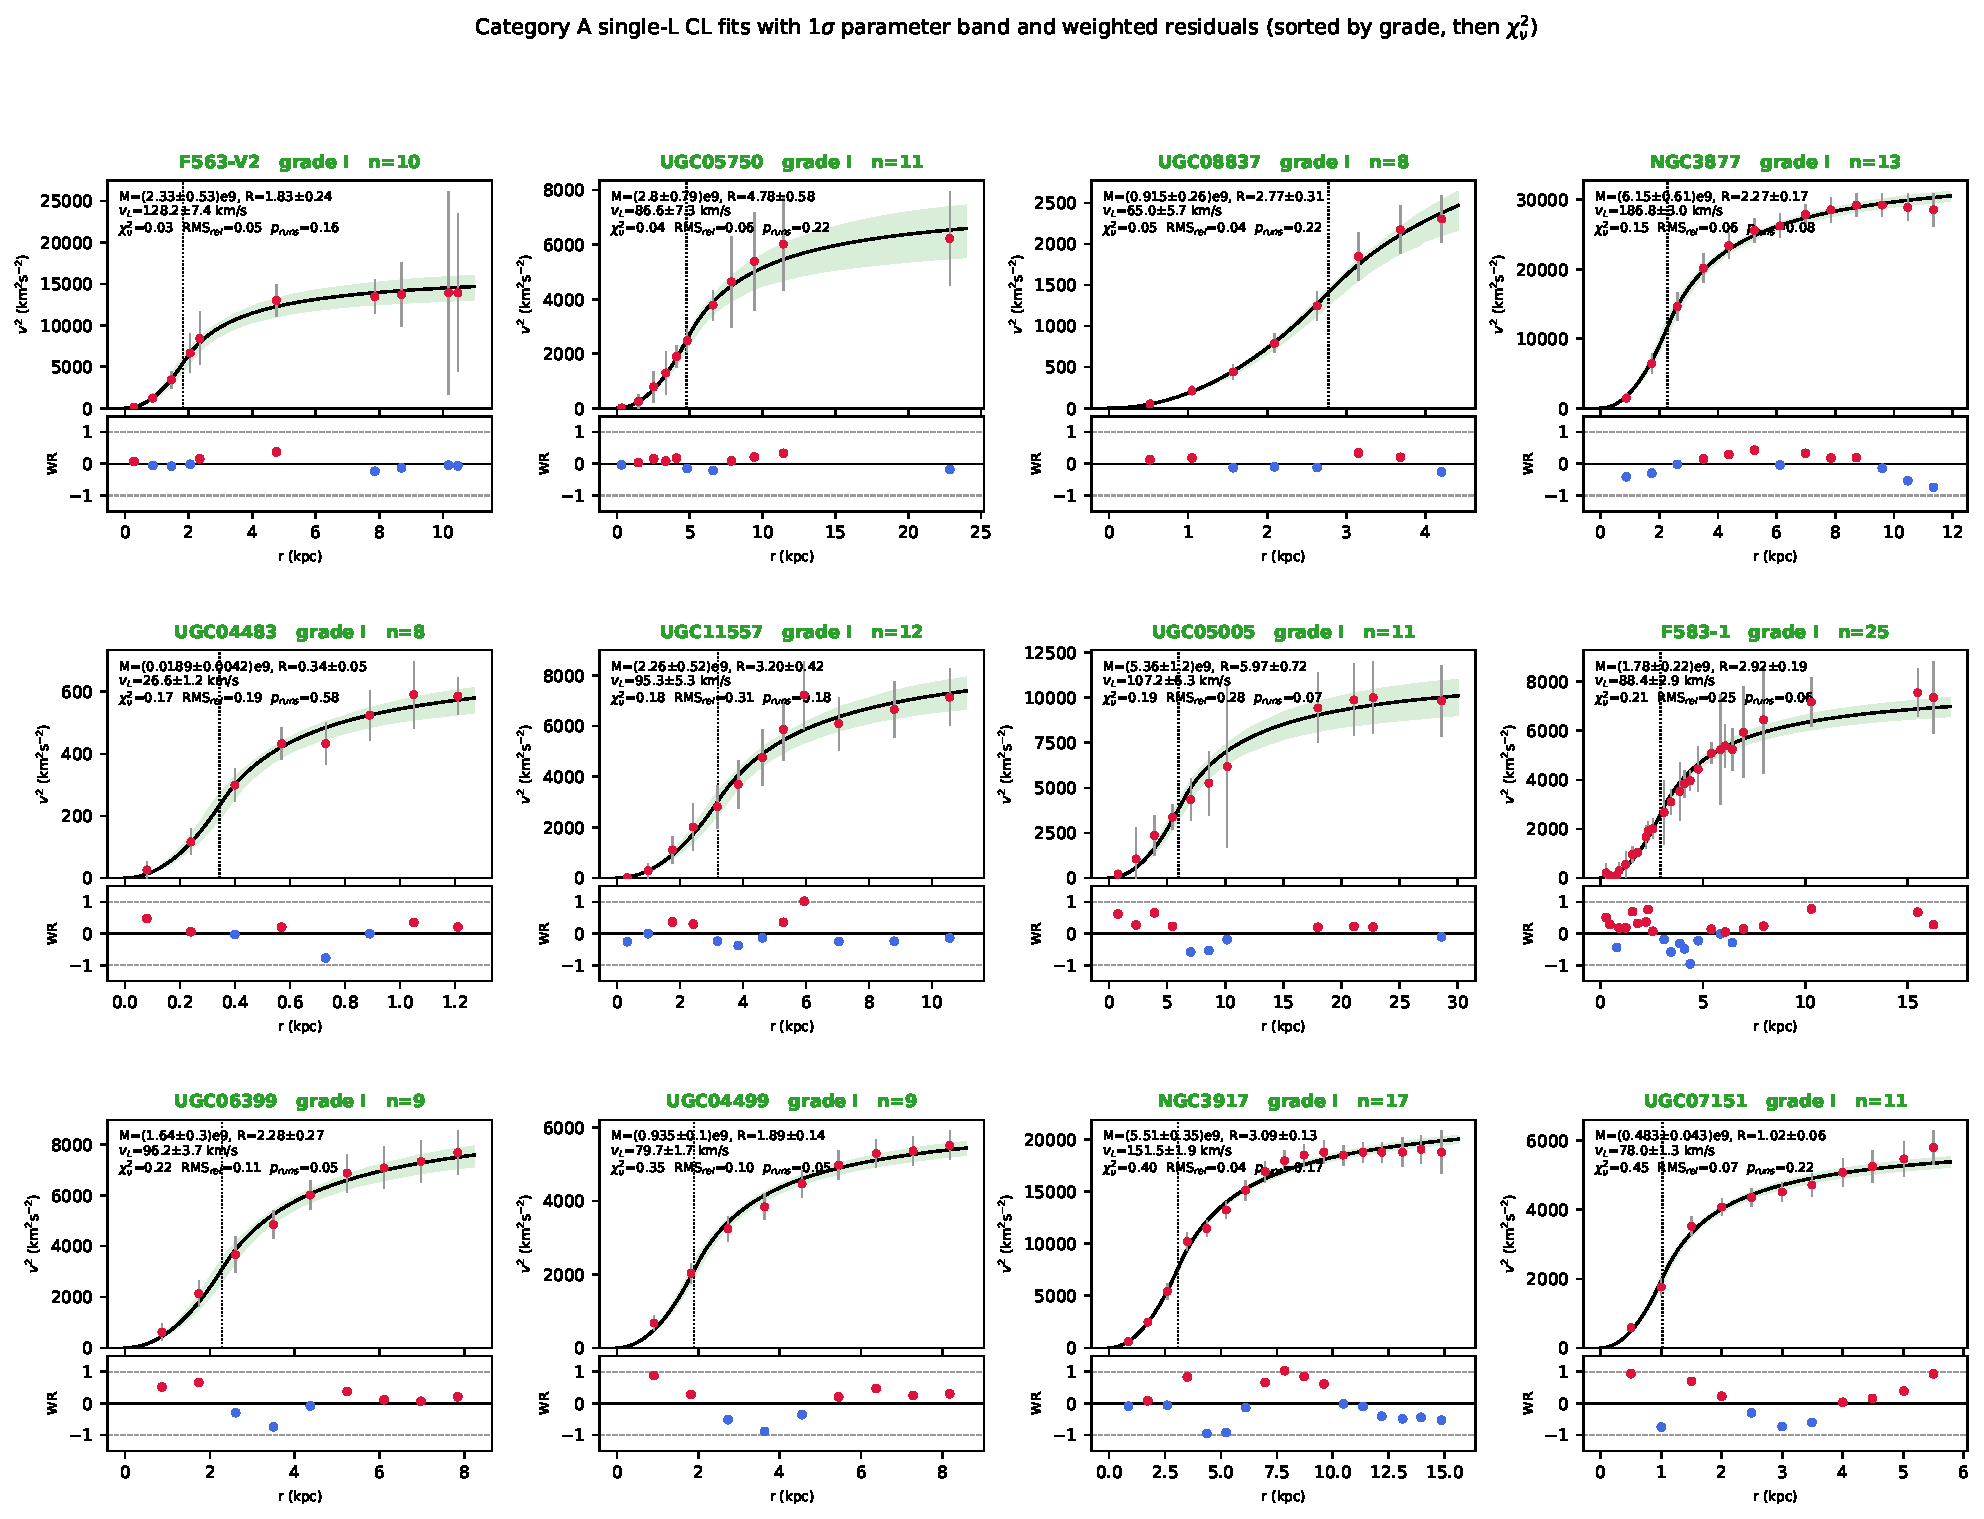
\includepdf[pages=-,landscape=true,scale=0.95]{catA_atlas.pdf}
\end{document}